\documentclass[crop,tikz]{standalone}

\begin{document}
  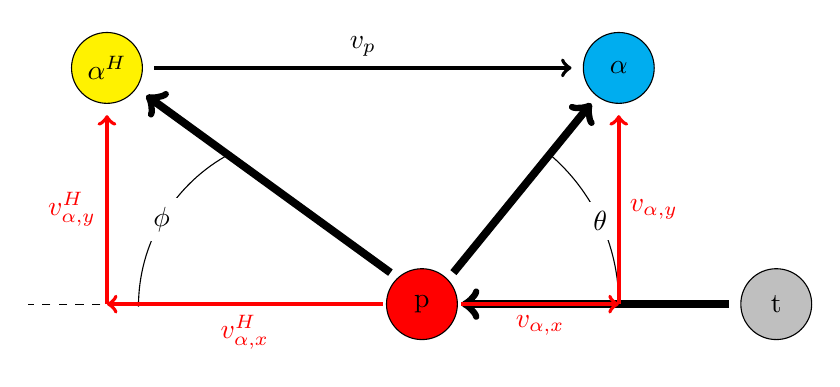
\begin{tikzpicture}
    \node[circle, draw, fill=red, minimum size = 0.9cm] (c) at (0,0){p}; 
    \draw [-to, line width=1mm] (3.9,0) -- (0.5,0);
    \node[circle, draw, fill=lightgray, minimum size = 0.9cm] (c) at (4.5,0){t}; 
    \node[circle, draw, fill=yellow, minimum size = 0.9cm] (c) at (-4,3){$\alpha^H$}; 
    \node[circle, draw, fill=cyan, minimum size = 0.9cm] (c) at (2.5,3){$\alpha$}; 
    \draw [-to, line width=1mm] (-0.4,0.4) -- (-3.5,2.65);
    \draw [-to, line width=1mm] (0.4,0.4) -- (2.15,2.55);
    \draw [-to, line width=0.5mm] (-3.4,3) -- (1.9,3) node[above,midway,fill=white] {$v_p$};
    \draw [dashed] (-0.5,0) -- (-5,0);
    \draw (2.5,0) arc [start angle=0, end angle=50, x radius=2.5cm, y radius =2.5cm] node[midway,fill=white] {$\theta$};
    \draw (-2.5,1.875) arc [start angle=120, end angle=180, x radius=2.2cm, y radius =2.2cm] node[midway,fill=white] {$\phi$};
    \draw [-to, line width=0.5mm,red] (-0.5,0) -- (-4,0) node[midway,below] {$v_{\alpha,x}^H$};
    \draw [-to, line width=0.5mm,red] (-4,0) -- (-4,2.4) node[midway,left] {$v_{\alpha,y}^H$};
    \draw [-to, line width=0.5mm,red] (0.5,0) -- (2.5,0) node[midway,below] {$v_{\alpha,x}$};
    \draw [-to, line width=0.5mm,red] (2.5,0) -- (2.5,2.4) node[midway,right] {$v_{\alpha,y}$};
  \end{tikzpicture}
\end{document}